\section{Выделение силуэта кисти руки}
\label{sec:Threholding}

Помимо классических методов определения границ можно использовать сегментацию по цвету кожи \cite{Phung}. Данный метод преобразует RGB изображение в бинарное с помощью фильтрации пикселей по цвету, близкому к цвету кожи. Для улучшения работы алгоритма перед фильтрацией изображение переводят в цветовое пространство YCrCb, в котором различные цвета кожи  расположены близко друг к другу \cite{Siddharth}.

Данный метод предусматривает обработку каждого пикселя независимо от других, проверяя его на принадлежность заданному диапазону. Это позволяет ускорить работу алгоритма реализацией параллельной обработки отдельных пикселей.

В большинстве случаев после бинаризации на изображении присутствуют шумы и артефакты, вызванные тем, что на фоновой части изображения находились пиксели, попадающие в ограничения фильтра. Для их устранения можно использовать морфологические операции: "наращивание" и "эрозия" \cite{DIP}:

Пусть имеется бинарное изображение A и структурный элемент B c началом координат в его центре (рисунок \ref{fig:morf}.)

	\begin{figure*}[!h]
	\centering
	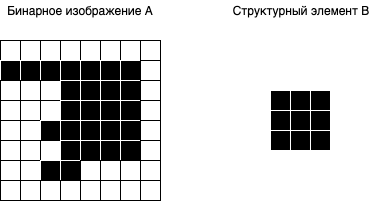
\includegraphics[,keepaspectratio]{figures/ru/morf}
	\caption{Бинарное изображение и структурный элемент}
	\label{fig:morf}
\end{figure*}

\begin{itemize}
	\item Наращивание. Задается как $A \oplus B = \cup_{b \in B}A_b$. Каждый раз, когда начало координат структурного элемента совмещается с единичным бинарным пикселем, ко всему структурному элементу применяется перенос и последующее логическое сложение с соответствующими пикселями бинарного изображения (рисунок \ref{fig:dil}).
	
	\begin{figure*}[!h]
		\centering
		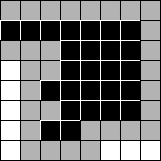
\includegraphics[,keepaspectratio]{figures/ru/dil}
		\caption{Наращивание бинарного изображения A структурным элементом B}
		\label{fig:dil}
	\end{figure*}
	
	\item Эрозия. Задается как $A \ominus B = \{ z \in A | B_z \subseteq A \}$. При выполнении операции эрозии структурный элемент тоже проходит по всем пикселям изображения. Если в некоторой позиции каждый единичный пиксель структурного элемента совпадет с единичным пикселем бинарного изображения, то выполняется логическое сложение центрального пикселя структурного элемента с соответствующим пикселем выходного изображения (рисунок \ref{fig:eros}).
	
	\begin{figure*}[!h]
		\centering
		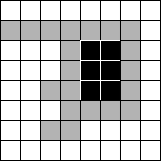
\includegraphics[,keepaspectratio]{figures/ru/eros}
		\caption{Эрозия бинарного изображения A структурным элементом B}
		\label{fig:eros}
	\end{figure*}
\end{itemize}